\chapter{Visualizing Neural Networks}

This exploration focuses on neural network visualization, a crucial aspect of understanding and analyzing how these models make decisions. It emphasizes the importance of interpretability and transparency in machine learning. Through the exploration of various visualization techniques, we can gain valuable insights into how these complex models interpret and process visual information. This endeavor helps bridge the divide between theoretical knowledge and real-world application, contributing to our deeper understanding of how neural networks function and their significance in modern AI solutions.

\section{Saliency Map}

This section focuses on identifying the most impactful pixels in an image for predicting its correct class. It employs a method proposed by Simonyan et al. (2014), which approximates the neural network around an image and visualizes the influence of each pixel.

\paragraph*{1. $ \bigstar $ Show and interpret the obtained results.}
In the process of visualizing multiple saliency maps, most of them exhibited consistent patterns, while some displayed inconsistencies. Let's examine each case.

% J'interprète souvent comme "le modèle regarde" alors que la saillancy map est que pour la class prédite et pas pour la ground truth faudrait visu les deux mais du coup pour limiter le nombre de figure mettre moins d'example ? 

In \Cref{fig:good_saliency_map}, we observe saliency maps that are generally consistent. When the model makes accurate predictions, we can observe high saliency values on the labeled object. This holds true for all the images in this figure, except for the fourth one where the model predicted "greenhouse" instead of "lakeside." In this case, the model did not focus on the lake boundaries, which led to the incorrect prediction. Instead, it primarily concentrated on the dark ground and the bright areas of the image, resulting in the "greenhouse" class prediction.

Now, in \Cref{fig:bad_saliency_map}, we encounter saliency maps that appear inconsistent. Both the first and fourth images are examples where the model's prediction is correct, but the corresponding saliency maps lack informativeness and appear blurry. In contrast, for the second and last images, the model seems to be focusing on the right regions, but it still predicts the wrong class.

\begin{figure}[H]
    \centering
    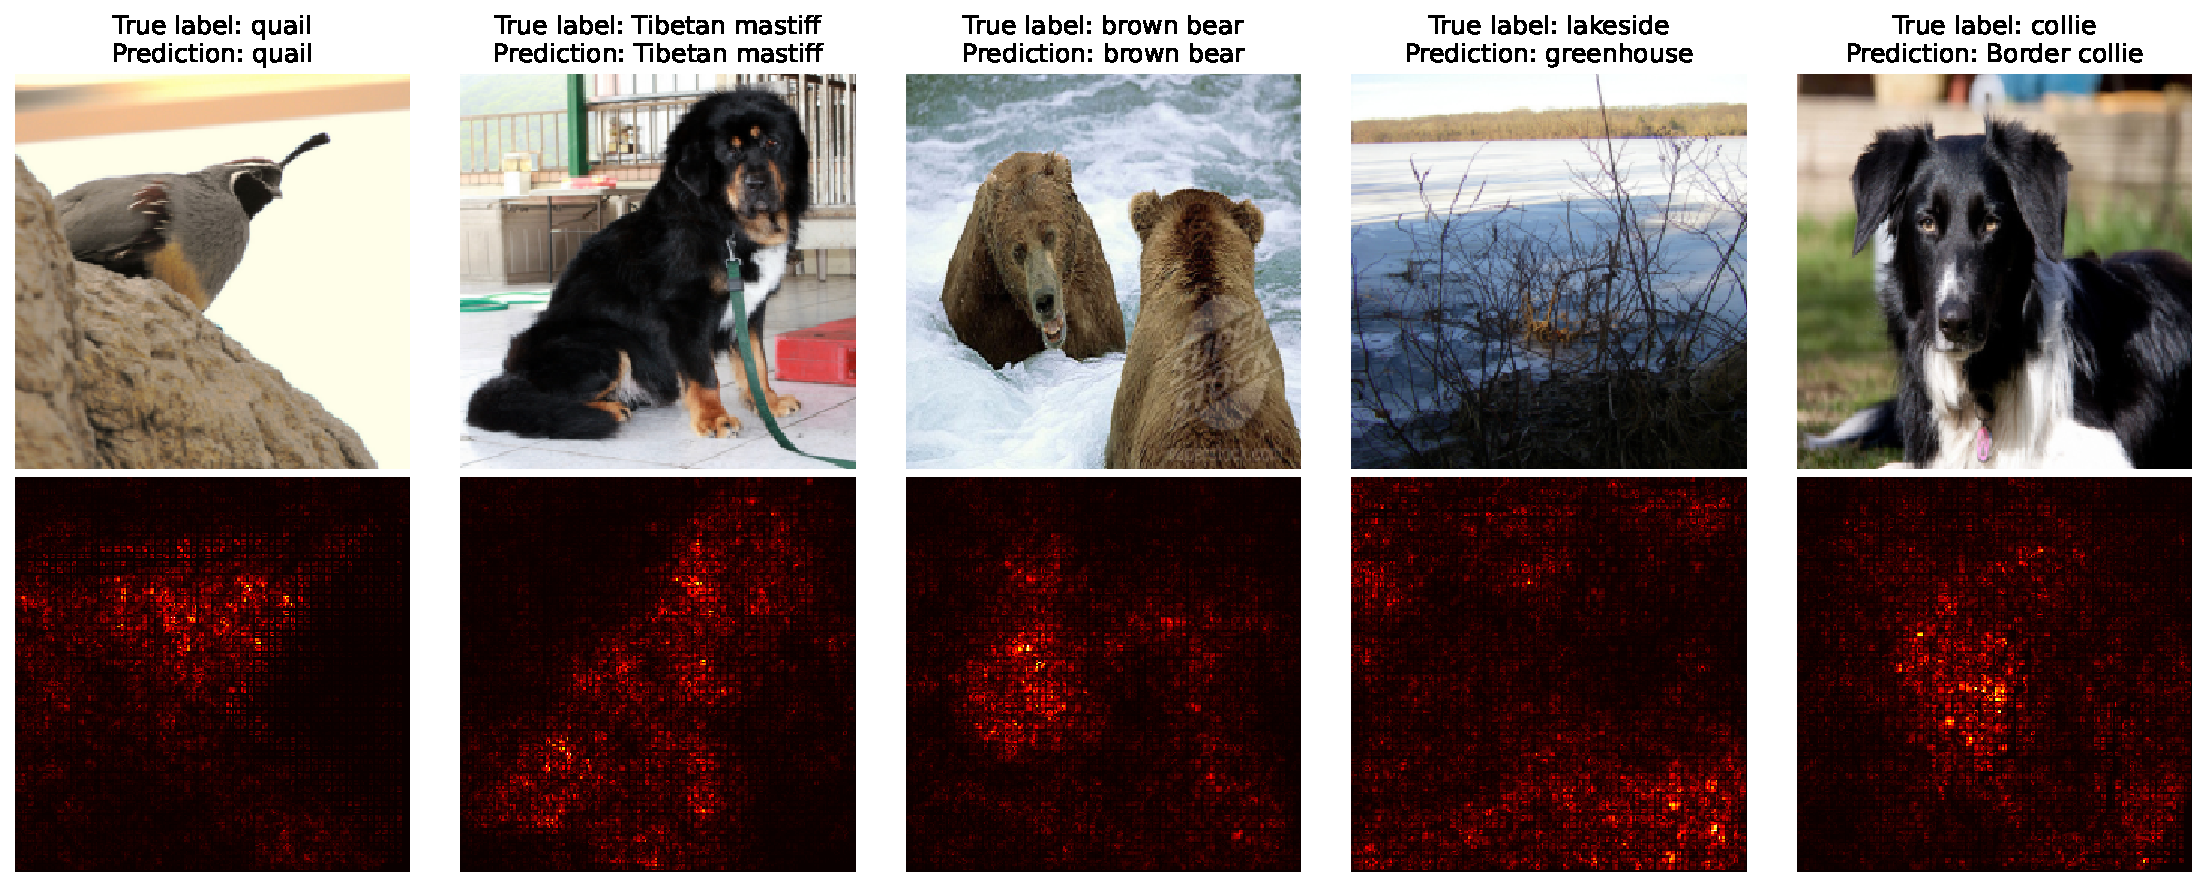
\includegraphics[width=.95\textwidth]{figs/2b/good_saliency_map.pdf}
    \caption{Consistent saliency maps of the predicted class}
    \label{fig:good_saliency_map}
\end{figure}

\begin{figure}[H]
    \centering  
    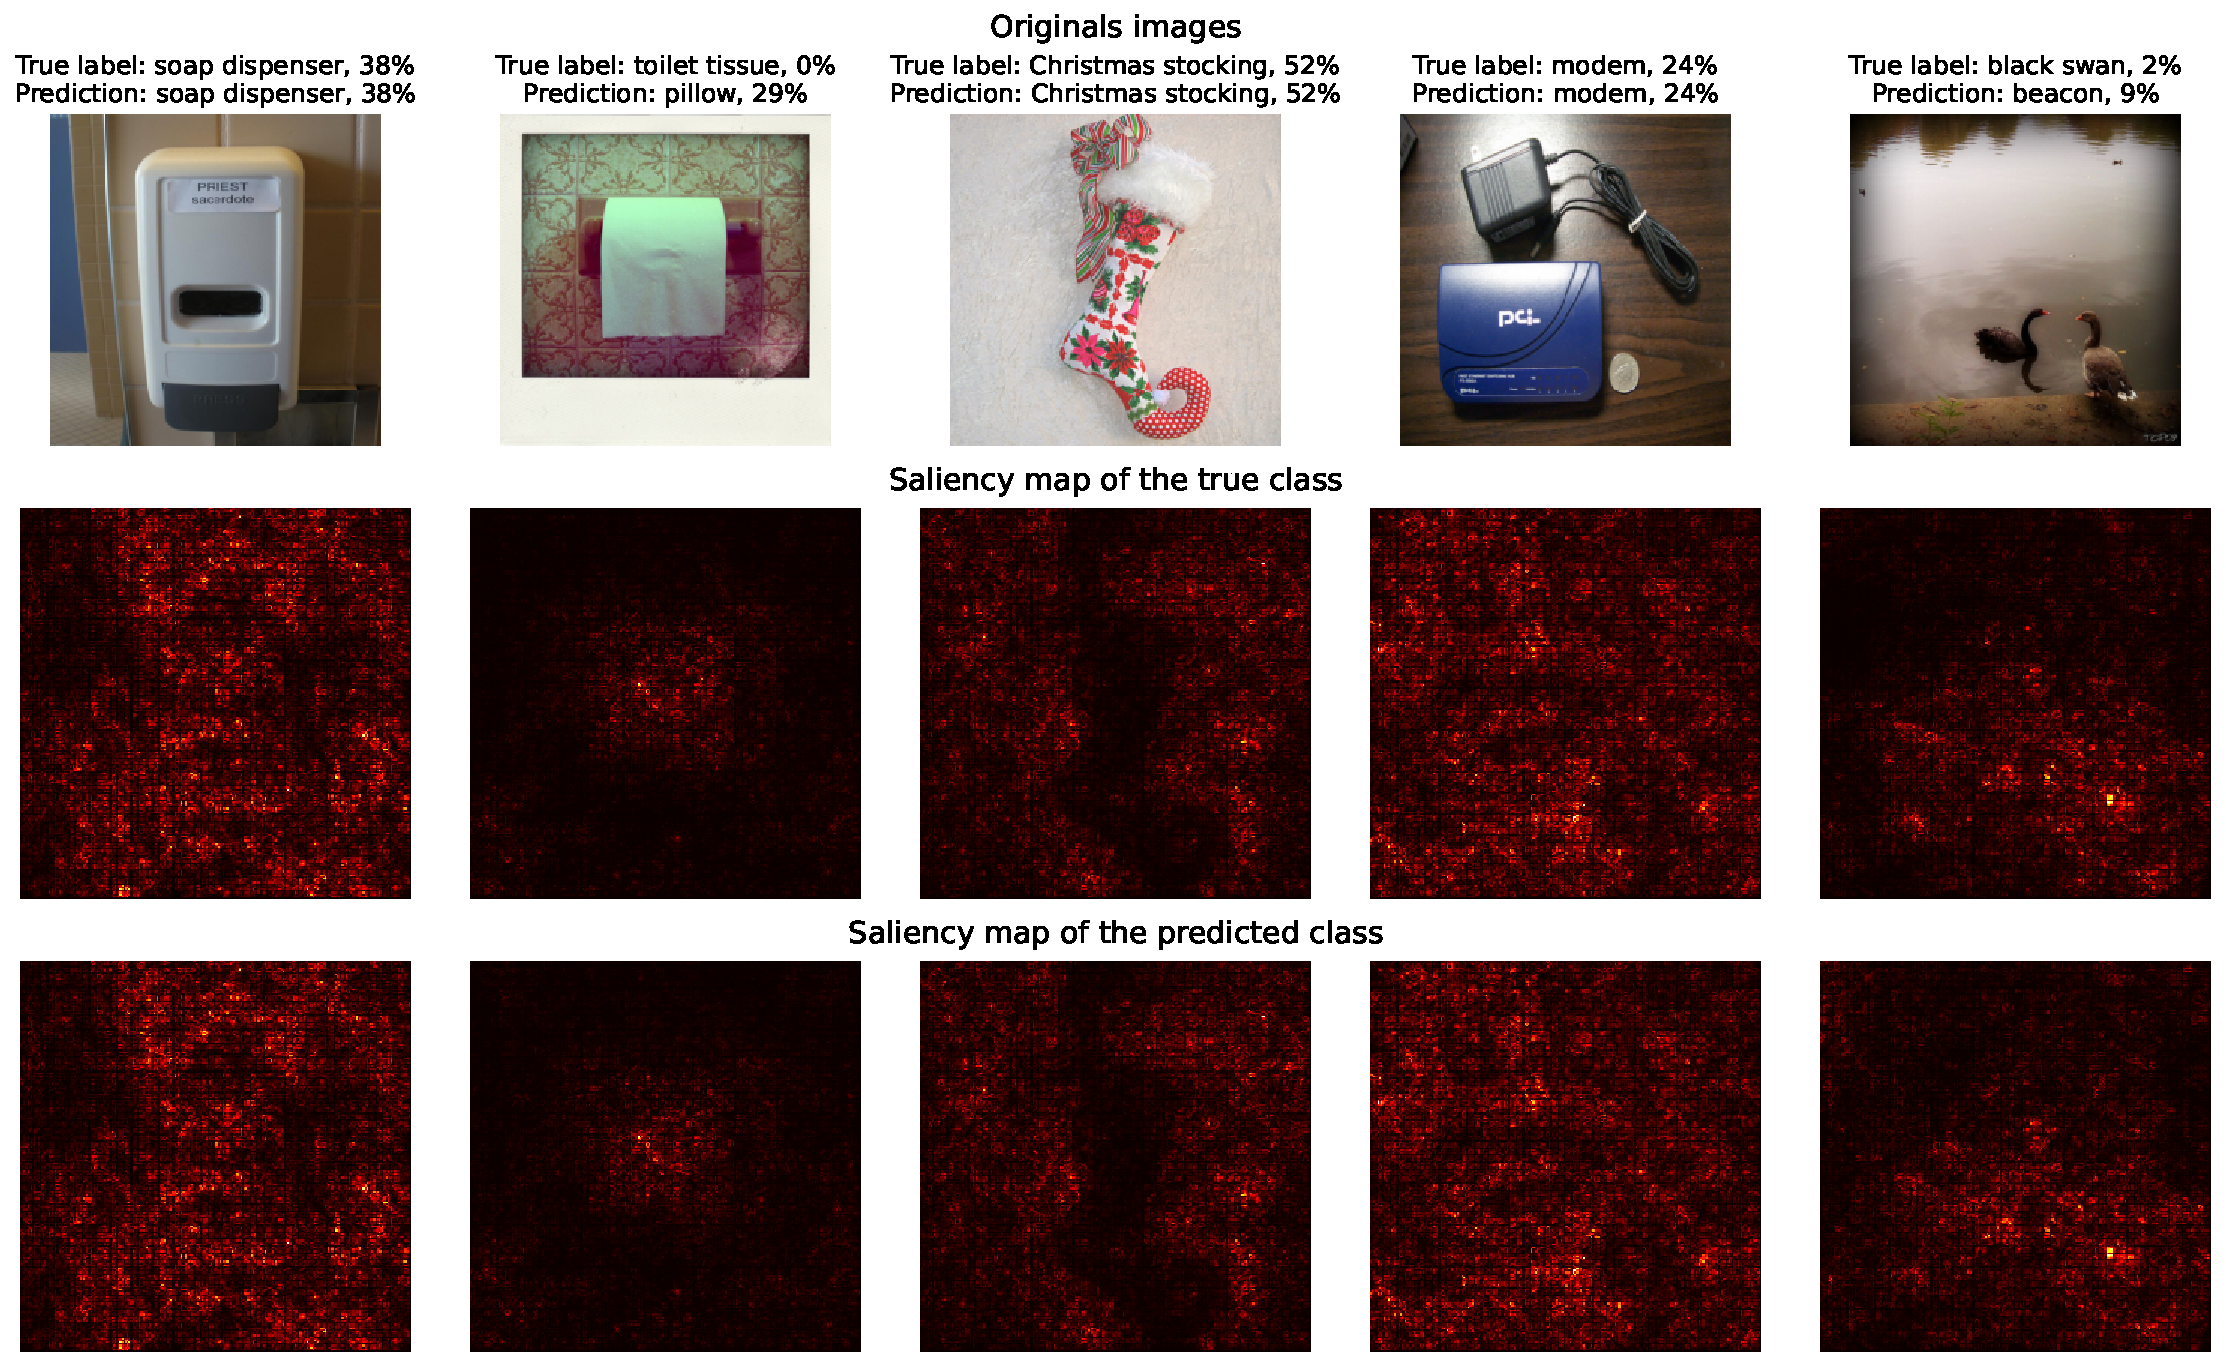
\includegraphics[width=.95\textwidth]{figs/2b/bad_saliency_map.pdf}
    \caption{Inconsistent saliency maps of the predicted class}
    \label{fig:bad_saliency_map}
\end{figure}

\paragraph*{2. Discuss the limits of this technique of visualization the impact of different pixels.}
As we discussed in the previous question, saliency maps can face challenges when dealing with images containing multiple objects or complex scenes. In such scenarios, these maps may become cluttered or unclear, making it challenging to extract meaningful insights. They can also suffer from noise or, conversely, overemphasize certain features while downplaying others. This can result in a biased interpretation of the model's focus.

Interpreting saliency maps can be subjective, especially when they are ambiguous. Different individuals may draw different conclusions from the same saliency map, resulting in inconsistent interpretations of the model's behavior. To gain a better understanding, we found it necessary to repeatedly analyze and visualize various saliency maps, particularly when they exhibited inconsistencies. It can be a complex task to keep in mind that each map represents the model's attention for a specific class, not the entire model. Examining saliency maps for other high-probability classes can provide additional context, contributing to a more complete understanding of the model's decision-making process.

It's important to note that saliency maps tend to highlight correlations rather than establishing causation. They reveal areas where the model directed its attention but do not necessarily imply that these areas directly influenced the model's decision.

\paragraph*{3. Can this technique be used for a different purpose than interpreting the network ?}
Saliency maps can be used to identify and localize important objects or regions in an image. This can be particularly useful in applications like automated image tagging or initial steps of object detection. This can also  help to create more effective augmented images by applying transformations (like rotations, scaling, cropping) that preserve these key areas. This technique is primarily suited for image data. Its utility is limited in non-visual domains or for models that integrate multiple types of data (like text and images).

%Feature Engineering and Selection: By identifying which parts of an input are most salient to a model's decision, saliency maps can inform feature engineering and selection in machine learning. This can be particularly useful in fine-tuning models by focusing on the most relevant features. ??????

\paragraph*{4. \textbf{Bonus:} Test with a diffrentent network, for example VGG16, and comment.}
% Guillaume a fait sur un ViT aussi
We tried the same saliency maps using VGG16. Those are much better! It  
% Make a comparaison plot for most of the "bad" saliency map, much better frontier, better classification also, Tibetan mastiff dog much clear frontiere too

\begin{figure}[H]
    \centering
    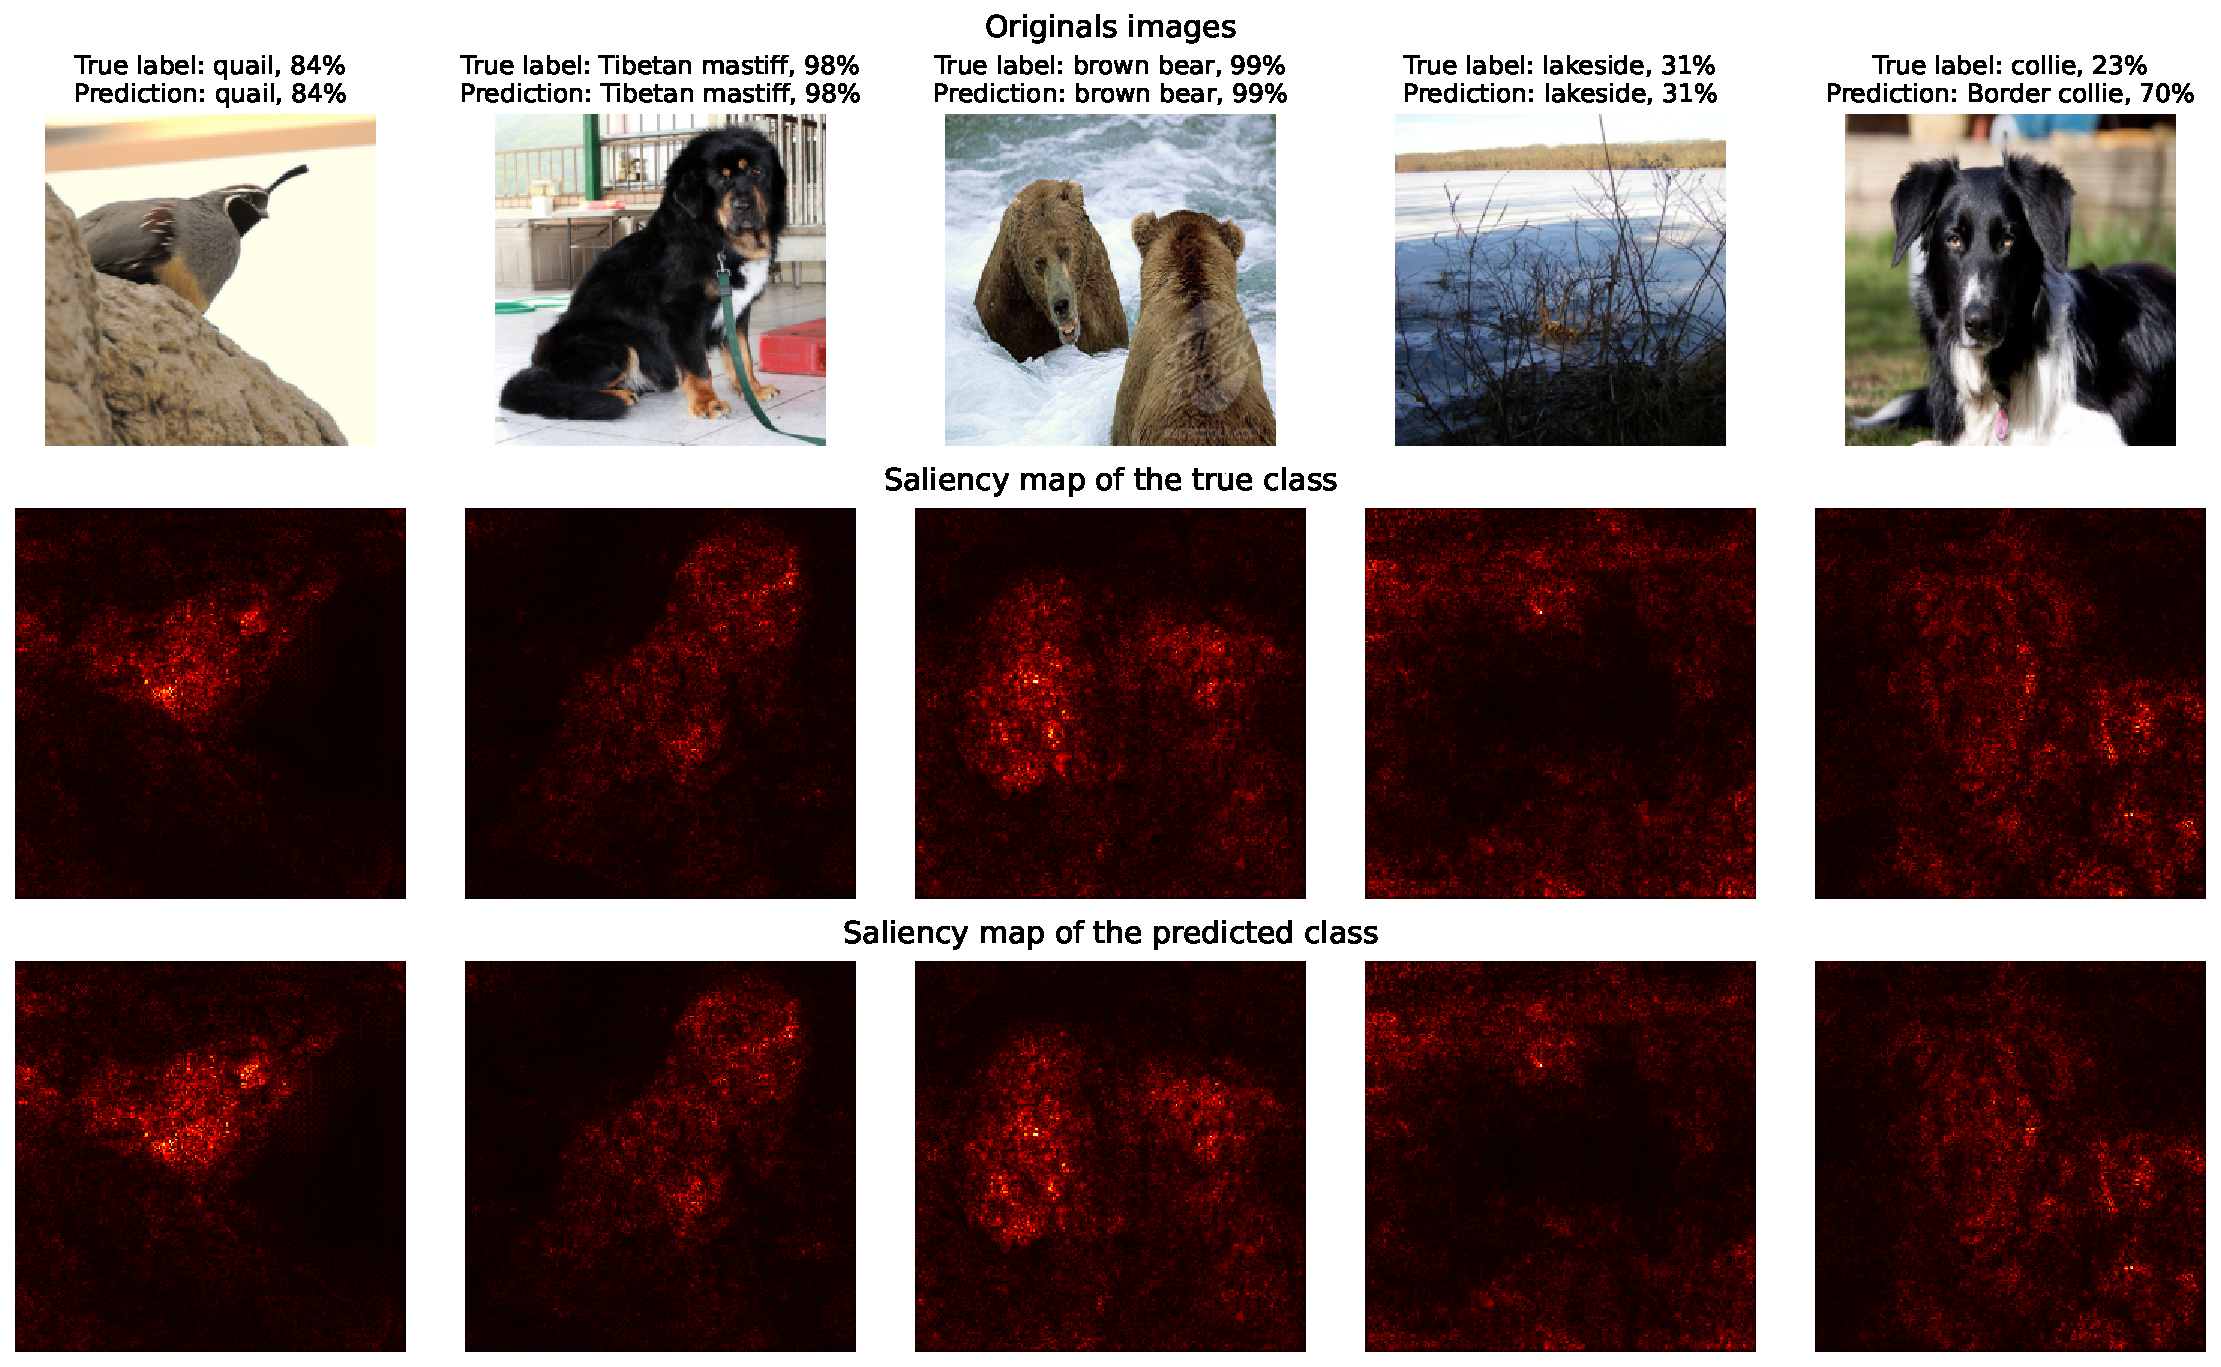
\includegraphics[width=.95\textwidth]{figs/2b/good_saliency_map_vgg16.pdf}
    \caption{Consistent saliency maps of the predicted class}
    \label{fig:good_saliency_map_vgg16}
\end{figure}

\begin{figure}[H]
    \centering  
    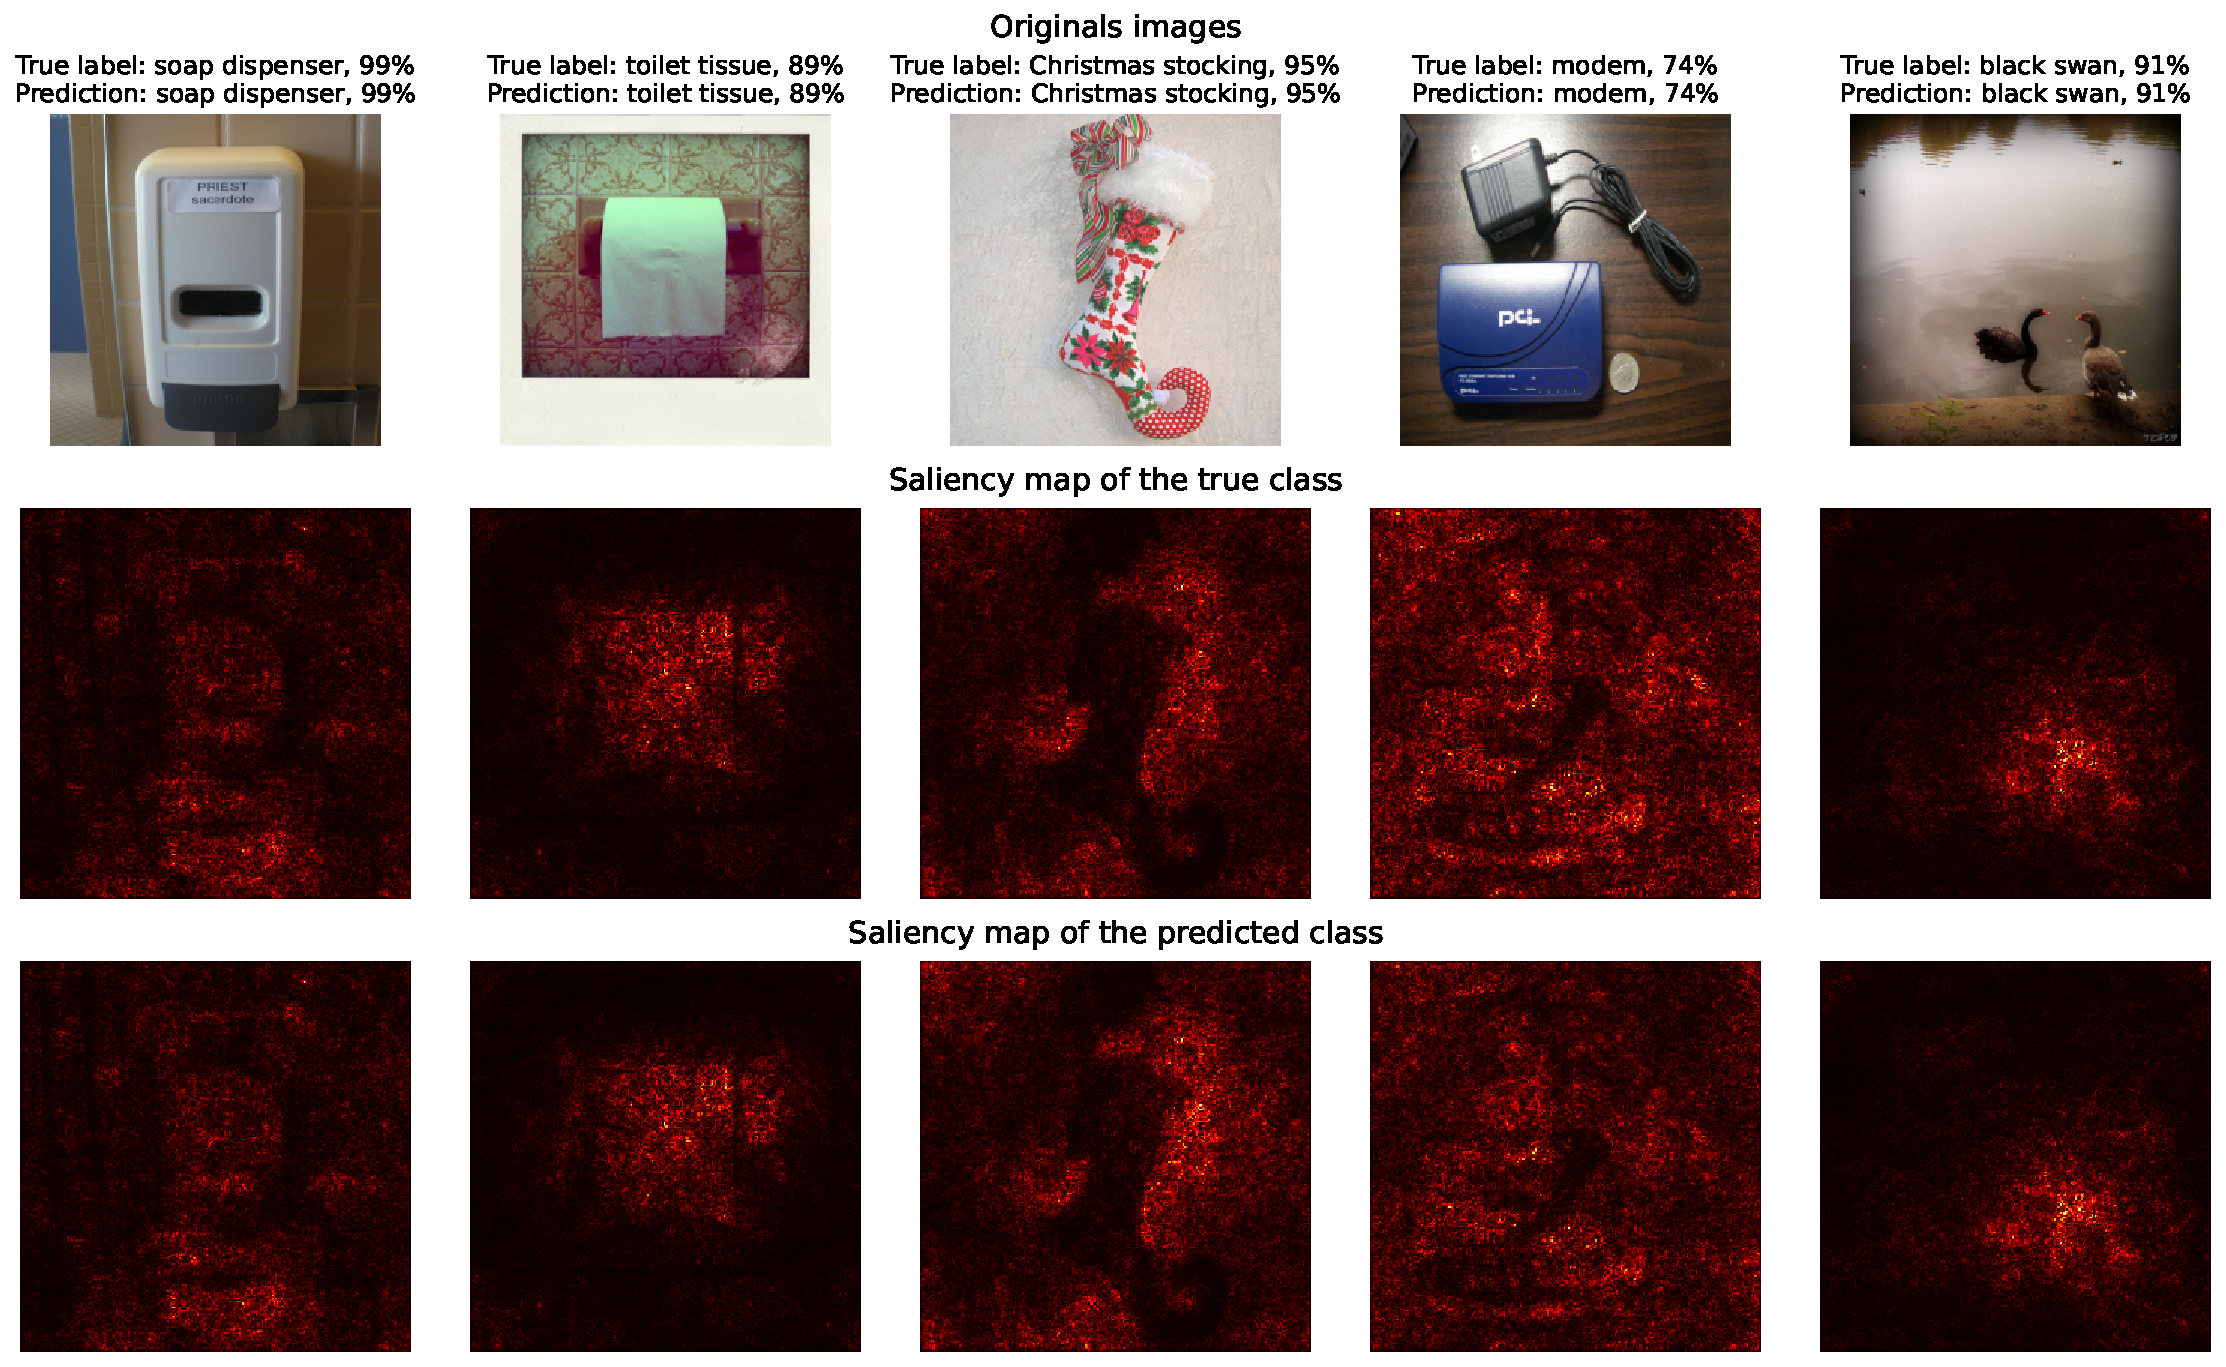
\includegraphics[width=.95\textwidth]{figs/2b/bad_saliency_map_vgg16.pdf}
    \caption{Inconsistent saliency maps of the predicted class}
    \label{fig:bad_saliency_map_vgg16}
\end{figure}


\section{Adversarial Example}

Here, the goal is to study the vulnerability of CNNs to minor, imperceptible modifications in an image that lead to misclassification. This concept, introduced by Szegedy et al. (2014), reveals the limitations and unexpected behaviors of neural networks.

\paragraph*{5. $ \bigstar $ Show and interpret the obtained results.}

\paragraph*{6. In practice, what consequences can this method have when using convolutional neural networks?}

\paragraph*{7. \textbf{Bonus:} Discuss the limits of this naive way to construct adversarial images. Can you propose some alternative or modified ways? (You can base these on recent research)}

\section{Class Visualization}

This section aims to generate images that highlight the type of patterns detected by a network for a particular class, based on techniques developed by \cite{simonyan2014deep} and \cite{yosinski2015understanding}. This method helps in visualizing what features the network prioritizes for classification. % trouver comment citer correctement ?? jpp 

\paragraph*{8. $ \bigstar $ Show and interpret the obtained results.}
Class visualization is a technique aimed at understanding what features or patterns a CNN has learned to recognize for a specific class. It involves generating an input image that maximally activates a class score in the network. Here, we've done this by iteratively modifying an initial random image to increase the activation of the desired class through gradient ascent on the class score with respect to the input image.

As a first try of this method, we decided to visualize our prefered animal : a wombat. \Cref{fig:class_viz_wombat} present a class visualization for a wombat after 1000 epochs and using the default regularization parameters in the given implementation (regularization factor of $1e^{-3}$, bluring every ten epoch, learning rate of $5$). 


\begin{figure}[H]
    \centering
    \begin{subfigure}{.5\textwidth}
        \centering
        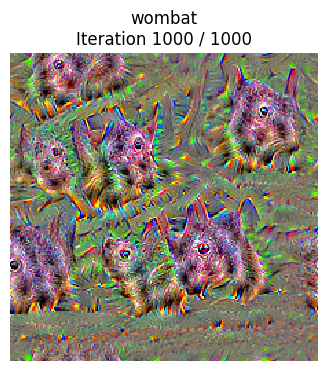
\includegraphics[width=.7\linewidth]{figs/2b/SqueezeNet/SqueezeNet_wombat_animated_1000_last_frame.png}
        \caption{Last iteration}
        \label{fig:class_viz_wombat:png}
    \end{subfigure}%
    \begin{subfigure}{.5\textwidth}
        \centering
        % \includemedia[width=.7\linewidth, height=.7\linewidth]{}{figs/2b/SqueezeNet/SqueezeNet_wombat_animated_1000.mp4}
        \caption{GIF animation (use Adobe Acrobat for viewing or see \textit{SqueezeNet\_wombat\_animated\_1000.mp4})}
        \label{fig:class_viz_wombat:vid}
    \end{subfigure}

    \caption{Class visualization: started from random noise, maximising the score from the wombat class. Using default regularization parameters (regularization factor of $1e^{-3}$, bluring every ten epoch, learning rate of $5$).}
    \label{fig:class_viz_wombat}
\end{figure}

\paragraph*{9. Try to vary the number of iterations and the learning rate as well as the regularization weight.}
When looking at some of our animation, we could see the bluering occuring every 10 steps.

To improve class visualization, it appears that regularization plays a crucial role. In \Cref*{fig:class_viz_reg}, we experimented with disabling image blurring and weight regularization on VGG16. Although we initially used a different model to achieve better visuals, all experiments were subsequently conducted on both SqueezeNet and VGG16.

% Non regulated images seem to be more saturated everywhere, preventing to clearly see the represented class. We suspect that without regularization, the gradient saturate \textbf{everypixel} that could ever had participate to a correct gorilla prediction. By promoting pixel which the model has already engaged the transformation and keeping this direction,regularization permit the arrival of real class image.

% Pas giga clair maybe 
Non-regularized images appear to be overly saturated, making it challenging to discern the represented class clearly. Our suspicion is that without regularization, gradients become saturated in \textbf{every pixel} that could have contributed to a correct prediction of "bee eater." By encouraging pixels that the model has already engaged in transformations and maintaining their direction, regularization facilitates the emergence of the true class image.

\begin{figure}[H]
    \centering
    \begin{subfigure}[t]{.33\textwidth}
        \centering
        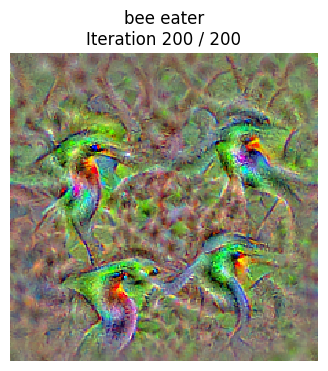
\includegraphics[width=\linewidth]{figs/2b/SqueezeNet/SqueezeNet_bird_animated_reg++_last_frame.png}
        \caption{With a lot of regularization}
        \label{fig:class_viz_reg:sub1}
    \end{subfigure}%
    \begin{subfigure}[t]{.33\textwidth}
        \centering
        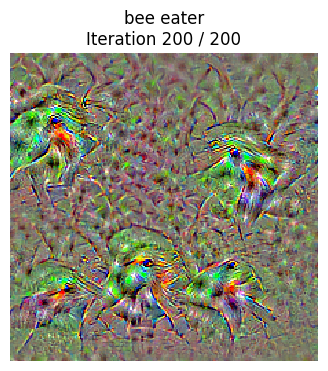
\includegraphics[width=\linewidth]{figs/2b/SqueezeNet/SqueezeNet_bird_animated_last_frame.png}
        \caption{With regularization}
        \label{fig:class_viz_reg:sub2}
    \end{subfigure}%
    \begin{subfigure}[t]{.33\textwidth}
        \centering
        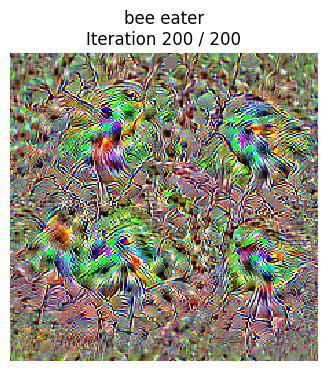
\includegraphics[width=\linewidth]{figs/2b/SqueezeNet/SqueezeNet_bird_animated_no_reg_last_frame.png}
        \caption{Without regularization}
        \label{fig:class_viz_reg:sub3}
    \end{subfigure}

    \caption{Comparaison of the bee eater class visualization using VGG16 with or without regularization (blurring and weight regularization) and starting from a base image of the class.}
    \label{fig:class_viz_reg}
\end{figure}

About the number of epoch, our experiment show that we need to make a certain number of epoch to let the visualization converge, thus getting better images.
\begin{figure}[H]
    \centering
    \begin{subfigure}[t]{.25\textwidth}
        \centering
        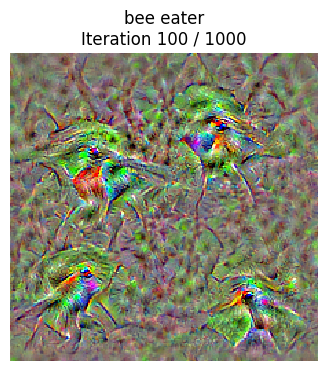
\includegraphics[width=\linewidth]{figs/2b/SqueezeNet/SqueezeNet_bird_animated_1000_regpp_blur_100_frame.png}
        \caption{200 iterations}
        \label{fig:class_viz_iter:sub1}
    \end{subfigure}%
    \begin{subfigure}[t]{.25\textwidth}
        \centering
        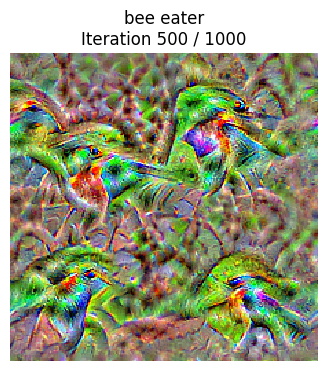
\includegraphics[width=\linewidth]{figs/2b/SqueezeNet/SqueezeNet_bird_animated_1000_regpp_blur_500_frame.png}
        \caption{500 iterations}
        \label{fig:class_viz_iter:sub2}
    \end{subfigure}%
    \begin{subfigure}[t]{.25\textwidth}
        \centering
        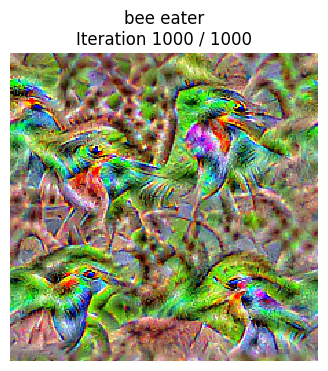
\includegraphics[width=\linewidth]{figs/2b/SqueezeNet/SqueezeNet_bird_animated_1000_regpp_blur_last_frame.png}
        \caption{1000 iterations}
        \label{fig:class_viz_iter:sub3}
    \end{subfigure}%
    \begin{subfigure}[t]{.25\textwidth}
        \centering
        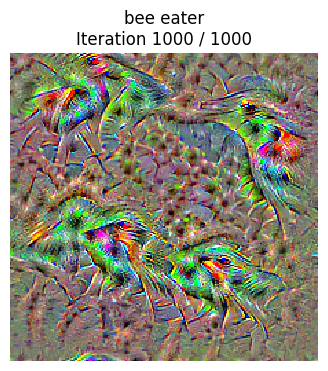
\includegraphics[width=\linewidth]{figs/2b/SqueezeNet/SqueezeNet_bird_animated_1000_last_frame.png}
        \caption{1000 iterations, no regularization}
        \label{fig:class_viz_iter:sub4}
    \end{subfigure}

    \caption{Same image at different time. The last one is another run but without regularization.}
    \label{fig:class_viz_iter}
\end{figure}

About the learning rate, TODO % TODO

\paragraph*{10. Try to use an image from ImageNet as the source image instead of a random image. You can use the real class as the target class. Comment on the interest of doing this.}

Starting using an image is a good method, it give a good starting point of the gradient to create visualization and not going everywhere like when not using regularization.
\begin{figure}[H]
    \centering
    \begin{subfigure}{.33\textwidth}
        \centering
        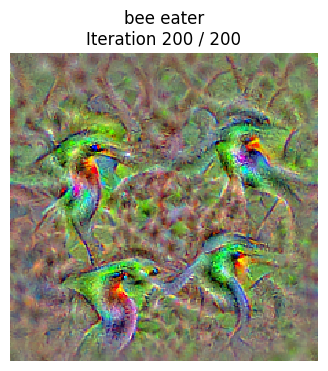
\includegraphics[width=.7\linewidth]{figs/2b/SqueezeNet/SqueezeNet_bird_animated_reg++_last_frame.png}
        \caption{Last iteration\\starting from noise}
        \label{fig:class_viz_start_image:png_noise}
    \end{subfigure}%
    \begin{subfigure}{.33\textwidth}
        \centering
        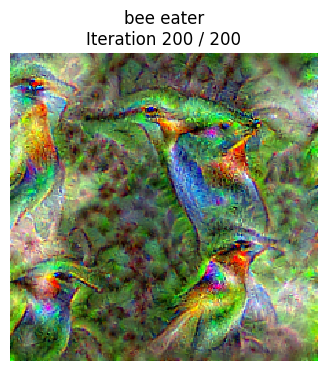
\includegraphics[width=.7\linewidth]{figs/2b/SqueezeNet/SqueezeNet_bird_animated_same_init_img_reg++_last_frame.png}
        \caption{Last iteration\\starting from same class}
        \label{fig:class_viz_start_image:png}
    \end{subfigure}%
    \begin{subfigure}{.33\textwidth}
        \centering
        % \includemedia[width=.7\linewidth, height=.7\linewidth]{}{figs/2b/SqueezeNet/SqueezeNet_bird_animated_same_init_img_reg++.gif}
        \caption{GIF animation\\starting from same class.} %(use Adobe Acrobat for viewing or see \textit{SqueezeNet\_bird\_animated\_same\_init\_img\_reg++.gif})}
        \label{fig:class_viz_start_image:vid}
    \end{subfigure}

    \caption{Class visualization: started from a bee eater image to maximising the score for the bee eater class. All with a strong regularization.}
    \label{fig:class_viz_start_image}
\end{figure}


It pretty funny to create some objects from other objects. In \Cref*{fig:class_viz_start_image_dif} we started from a image of hays to do a snail class visualization.
\begin{figure}[H]
    \centering
    \begin{subfigure}{.5\textwidth}
        \centering
        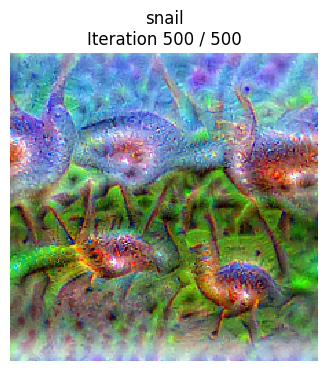
\includegraphics[width=.7\linewidth]{figs/2b/SqueezeNet/SqueezeNet_snail_animated_init_img_reg++_last_frame.png}
        \caption{Last iteration}
        \label{fig:class_viz_start_image_dif:png}
    \end{subfigure}%
    \begin{subfigure}{.5\textwidth}
        \centering
        % \includemedia[width=.7\linewidth, height=.7\linewidth]{}{figs/2b/SqueezeNet/SqueezeNet_snail_animated_init_img_reg++.gif} 
        \caption{GIF animation (use Adobe Acrobat for viewing or see \textit{.gif})}
        \label{fig:class_viz_start_image_dif:vid}
    \end{subfigure}

    \caption{Class visualization: started from a hay image to maximising the score for the snail class. All with a strong regularization.}
    \label{fig:class_viz_start_image_dif}
\end{figure}

\paragraph*{11. \textbf{Bonus:} Test with another network, VGG16, for example, and comment on the results.}
We did the all same experiment using VGG16 this time. Visualization are much better because of the overall better performance of VGG16 as we saw in \Cref{}. % Maybe ref la figure saliency map avec VGG16 où il se trompe pas


% Parfois plus délicat de faire des bonne visualization, mais le résultat est clairement plus clair, on voit que le réseau est plus performant que l'autre 